\section{RESULTADOS}\label{sec:resultados}

\subsection{Estatísticas descritivas}

A Tabela~\ref{tab:descritivas} resume as principais variáveis em valores reais per capita, a preços de 2025. Camaçari arrecada mais e produz mais: sua receita corrente per capita média é de R\$~6.610, contra R\$~5.034 em Barreiras, e seu PIB per capita é 2,3 vezes maior (R\$~116.253 contra R\$~49.473, até 2023). A distância se amplia na arrecadação própria, que soma R\$~1.554 per capita em IPTU, ISS e ITBI em Camaçari e R\$~505 em Barreiras, e na cota-parte do ICMS, de R\$~2.168 contra R\$~874. O FPM per capita inverte a ordem: é quase o dobro em Barreiras (R\$~1.032 contra R\$~547), porque o valor total é o mesmo e a população, a metade.

\begin{table}[H]
\centering\footnotesize
\setlength{\tabcolsep}{4pt}
\caption{Estatísticas descritivas: valores reais per capita, Barreiras e Camaçari (2016--2025)}
\label{tab:descritivas}
\begin{adjustbox}{max width=\textwidth}
\begin{tabular}{lrrrrrrrr}
\toprule
 & \multicolumn{4}{c}{Barreiras} & \multicolumn{4}{c}{Camaçari} \\
\cmidrule(lr){2-5}\cmidrule(lr){6-9}
R\$ de 2025 per capita & Média & DP & Mín. & Máx. & Média & DP & Mín. & Máx. \\
\midrule
Receita corrente & 5.034 & 794 & 3.781 & 6.155 & 6.610 & 687 & 5.593 & 7.519 \\
Impostos próprios$^{b}$ & 505 & 143 & 286 & 739 & 1.554 & 359 & 1.093 & 1.993 \\
Transf. incondicionais$^{c}$ & 2.105 & 418 & 1.645 & 2.746 & 2.827 & 140 & 2.651 & 3.014 \\
\quad FPM & 1.032 & 153 & 855 & 1.248 & 547 & 83 & 441 & 666 \\
\quad Cota-parte do ICMS & 874 & 236 & 573 & 1.249 & 2.168 & 180 & 1.888 & 2.410 \\
FUNDEB & 918 & 207 & 684 & 1.257 & 676 & 90 & 572 & 808 \\
Despesa total & 4.864 & 895 & 3.361 & 5.853 & 6.458 & 923 & 4.967 & 7.899 \\
\quad Educação & 1.502 & 313 & 944 & 1.910 & 1.387 & 217 & 1.108 & 1.697 \\
\quad Saúde & 1.334 & 207 & 975 & 1.613 & 1.207 & 151 & 983 & 1.419 \\
PIB per capita$^{a}$ & 49.473 & 10.975 & 33.846 & 63.025 & 116.253 & 11.016 & 96.979 & 137.715 \\
\bottomrule
\end{tabular}
\end{adjustbox}
\par\vspace{3pt}\parbox{\textwidth}{\scriptsize Nota: 10 observações anuais por município, exceto (a) PIB, disponível até 2023 (8 anos). Valores deflacionados pela média anual do IPCA (preços de 2025) e divididos pela população (estimativas do IBGE; Censo 2022 em 2022 e interpolação linear em 2023). (b) IPTU + ISS + ITBI. (c) FPM + ITR + cotas-partes de ICMS, IPVA e IPI-exportação + IOF-ouro. Despesa: empenhada. DP = desvio-padrão. Fonte: elaboração própria com dados do Siconfi (DCA) e do IBGE.}
\end{table}


Apesar da receita menor, Barreiras gasta mais per capita em educação (R\$~1.502 contra R\$~1.387) e em saúde (R\$~1.334 contra R\$~1.207). As vinculações constitucionais não explicam a diferença, porque incidem sobre a receita de impostos e transferências, maior por habitante em Camaçari. O peso maior do FUNDEB em Barreiras (R\$~918 per capita, contra R\$~676) sugere uma explicação demográfica, com mais matrículas por habitante, mas os dados deste trabalho não incluem a composição etária nem as matrículas, e a questão fica em aberto. As trajetórias também divergem. Entre 2016 e 2025, a receita corrente real per capita de Barreiras cresceu 62\% (de R\$~3.781 para R\$~6.116), e a de Camaçari, 22\% (de R\$~5.820 para R\$~7.073). A despesa acompanhou o movimento, e a distância entre os dois municípios diminuiu.

\subsection{Composição das receitas e dependência de transferências}

É na composição das receitas que a tese do artigo se verifica (Tabela~\ref{tab:composicao} e Figura~\ref{fig:fontes}). Com o mesmo FPM, a importância do fundo difere por um fator de dois a três: ele financia de 20\% a 25\% da receita corrente de Barreiras e de 7,7\% a 9,4\% da de Camaçari, nos anos da tabela. Considerado o conjunto das transferências correntes, a dependência de Barreiras fica entre 78\% e 82\% da receita corrente de 2016 a 2025, salvo em 2017 (e entre 84\% e 85\% em 2014 e 2015), contra 56\% a 65\% em Camaçari, com tendência de queda neste último. Em base líquida da dedução para o FUNDEB, que evita contar duas vezes os recursos retidos e devolvidos pelo fundo, as faixas nos anos da tabela caem para 76\% a 80\% e 52\% a 61\%, e a ordem não se altera. Pela medida contábil, a hipótese H2 se confirma; para o FPM, o resultado é quase mecânico, porque o valor é o mesmo e a receita de Barreiras é menor.

\begin{table}[H]
\centering\footnotesize
\setlength{\tabcolsep}{4pt}
\caption{Composição da receita corrente: participação de cada fonte (\% da receita corrente)}
\label{tab:composicao}
\begin{adjustbox}{max width=\textwidth}
\begin{tabular}{lrrrrrrrr}
\toprule
 & \multicolumn{4}{c}{Barreiras} & \multicolumn{4}{c}{Camaçari} \\
\cmidrule(lr){2-5}\cmidrule(lr){6-9}
Fonte & 2016 & 2019 & 2022 & 2025 & 2016 & 2019 & 2022 & 2025 \\
\midrule
FPM & 24,8\% & 20,8\% & 22,6\% & 20,4\% & 8,8\% & 7,7\% & 8,7\% & 9,4\% \\
Cota-parte do ICMS & 15,1\% & 15,8\% & 18,6\% & 20,4\% & 37,4\% & 38,2\% & 30,9\% & 26,8\% \\
Transf. incondicionais & 44,0\% & 40,6\% & 45,2\% & 44,9\% & 48,1\% & 47,6\% & 41,1\% & 37,9\% \\
Transf. correntes (total) & 82,0\% & 77,7\% & 78,8\% & 79,2\% & 64,8\% & 62,4\% & 58,1\% & 55,7\% \\
Transf. correntes, líquidas da dedução$^{a}$ & 80,4\% & 75,8\% & 76,8\% & 77,2\% & 61,0\% & 58,5\% & 54,5\% & 52,2\% \\
Transf. correntes sem a cota do ICMS$^{b}$ & 66,9\% & 61,9\% & 60,2\% & 58,7\% & 27,4\% & 24,2\% & 27,2\% & 28,9\% \\
Impostos próprios & 8,8\% & 10,6\% & 11,0\% & 10,9\% & 18,8\% & 21,6\% & 27,1\% & 27,8\% \\
Receita tributária & 13,5\% & 15,8\% & 16,4\% & 17,0\% & 23,7\% & 27,5\% & 33,3\% & 34,2\% \\
\bottomrule
\end{tabular}
\end{adjustbox}
\par\vspace{3pt}\parbox{\textwidth}{\scriptsize Nota: razões calculadas com valores nominais do mesmo ano. A receita corrente é bruta (inclui as transferências do FUNDEB antes da dedução). (a) Transferências correntes menos a dedução para o FUNDEB, divididas pela receita corrente também líquida da dedução, para não contar duas vezes os 20\% retidos do FPM e das cotas e devolvidos pelo fundo. (b) Transferências correntes menos a cota-parte do ICMS, divididas pela receita corrente. Anos selecionados do período 2016--2025. Em 2017, Barreiras registrou R\$ 178,6 milhões em ``Outras Transferências Multigovernamentais'', que elevam a participação das transferências naquele ano (não exibido). Fonte: elaboração própria com dados do Siconfi (DCA, Anexo I-C).}
\end{table}


\begin{figure}[H]
  \centering
  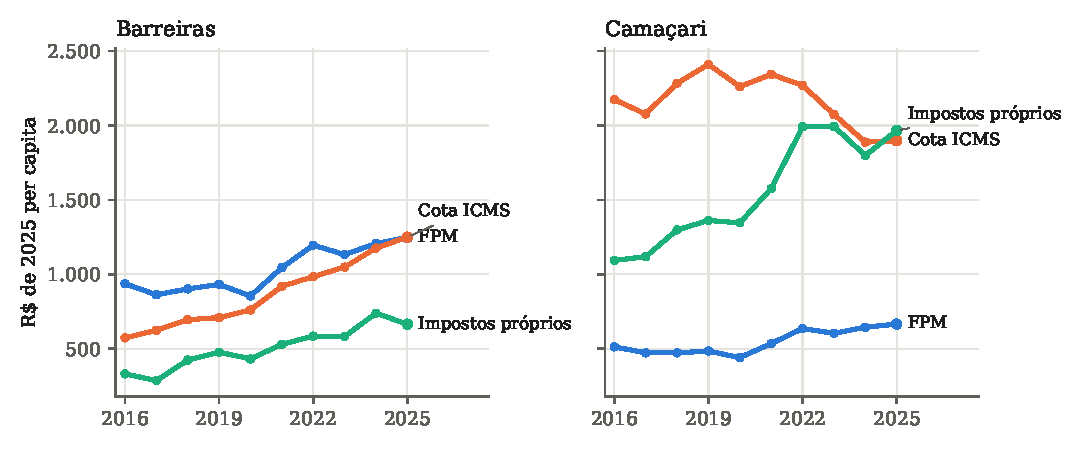
\includegraphics[width=\textwidth]{figuras/fig_fontes_receita.pdf}
  \caption{FPM, cota-parte do ICMS e impostos próprios: valores reais per capita (R\$~de 2025)}
  \label{fig:fontes}
  \fonte{elaboração própria com dados do Siconfi (DCA) e do IBGE.}
\end{figure}

O quadro muda quando a medida se restringe às transferências incondicionais. Em proporção da receita corrente, elas representam de 41\% a 45\% em Barreiras e de 38\% a 48\% em Camaçari nos anos da tabela, e as séries se cruzam: a diferença entre os dois nunca passa de 7 pontos percentuais e muda de sinal no período, com Camaçari acima em 2016 e 2019 e abaixo em 2022 e 2025. A semelhança vale como participação na receita, não em valor: por habitante, Camaçari recebe em média 34\% mais transferências incondicionais (R\$~2.827 contra R\$~2.105). Ela decorre da cota-parte do ICMS, que chegou a 38\% da receita corrente de Camaçari em 2019 e responde, em média, por 77\% de suas transferências incondicionais entre 2016 e 2025, contra 41\% em Barreiras. A hipótese H2 é confirmada para a dependência total e para o FPM, mas não para as transferências incondicionais, em que os municípios se alternam.

Retirada a cota do ICMS, a medida conta outra história (última linha da Tabela~\ref{tab:composicao}). As transferências correntes sem a cota financiam de 24\% a 30\% da receita corrente de Camaçari, contra 59\% a 67\% em Barreiras entre 2016 e 2025, salvo 2017, e a distância entre os dois passa de 15 a 24 para 29 a 40 pontos percentuais. O indicador convencional ordena corretamente o par, mas mais que dobra a dependência de Camaçari em relação a recursos sem vínculo com sua economia, porque conta como transferência uma receita gerada por sua própria indústria. É nesse sentido que a dependência registrada não acompanha a autonomia (H4): ela erra o nível de quem tem a receita vinculada à base local, ainda que acerte a ordem. O resultado é coerente com a conclusão de \citet{Franek2026518} de que a autonomia e a retenção da receita marginal importam mais do que a classificação formal da receita.

A cota do ICMS também acompanha a base local em Barreiras, o que impede tratá-la ali como repasse puramente redistributivo. Entre 2016 e 2025, a cota real per capita do município mais que dobrou, de R\$~573 para R\$~1.249, e em 2025 igualou o FPM por habitante. O movimento pode refletir a expansão do agronegócio no oeste baiano, mas também a parcela da cota repartida por critérios educacionais após a EC n.º 108/2020; o índice de participação publicado pela Secretaria da Fazenda da Bahia permitiria separar os dois efeitos. Em Camaçari, ao contrário, a cota caiu de R\$~2.174 em 2016 para R\$~1.897 em 2025, enquanto os impostos próprios subiram de 19\% para 28\% da receita corrente. A queda tem candidatos óbvios que os dados não permitem separar: o encerramento da produção da Ford no município, em 2021, que reduziu o valor adicionado industrial e, com defasagem, o índice de participação; a limitação do ICMS sobre combustíveis, energia e comunicações, em 2022, que reduziu a arrecadação estadual \citep{LC194}; e as mudanças nos critérios de repartição após a EC n.º 108/2020. A literatura admite duas leituras para a substituição de transferências por arrecadação própria: as duas fontes podem tanto se substituir \citep{DaCosta2016, Taiwo202231} quanto se complementar \citep{Masaki2018173, Porto2023642}. Em Barreiras, os impostos próprios cresceram, mas permanecem em torno de 11\% da receita corrente, o que é compatível com a menor capacidade fiscal do município \citep{dosSantos2017}. A outra face dessa vinculação é distributiva: a regra que devolve o ICMS a quem produz mais dá mais recursos a quem já tem mais base, padrão que a literatura associa às transferências devolutivas \citep{daCosta2024}.

\subsection{Gasto, transferências e PIB: efeitos marginais}

Se a dependência registrada mede mal a autonomia, resta saber se o gasto responde às transferências como prevê o efeito \textit{flypaper}. A Tabela~\ref{tab:regressao} apresenta as estimativas da equação~\eqref{eq:flypaper} em níveis per capita, em que os coeficientes são efeitos marginais em reais. Pelo critério correto da equivalência, o padrão é nítido. Na despesa total (1), cada real adicional de transferência incondicional associa-se a R\$~1,85 de gasto, e cada real adicional de PIB, a um valor estatisticamente nulo ($-$R\$~0,02); a diferença, de R\$~1,87, é significativa ($p = 0{,}014$), com intervalo de confiança de 95\% entre R\$~0,43 e R\$~3,32. Na despesa corrente (2), a diferença é de R\$~1,69 ($p = 0{,}004$). O coeficiente do PIB não se distingue de zero na despesa total, mas é negativo e significativo a 10\% na despesa corrente (2 e 4), e em reais é impreciso: na especificação (1), o intervalo de 95\% para o efeito de um desvio-padrão do PIB per capita (cerca de R\$~11 mil) vai de cerca de $-$R\$~600 a $+$R\$~170. Com $T^{*}$, que exclui a cota do ICMS, os efeitos marginais sobem para cerca de R\$~3 por real (3 e 4), e a diferença em relação ao PIB permanece significativa. A separação entre FPM e ICMS (5) mostra um coeficiente maior para o FPM (R\$~2,94) do que para o ICMS (R\$~0,63), mas a igualdade entre os dois não é rejeitada ($p = 0{,}21$): os dados não sustentam que o gasto responda de modo diferente às duas receitas.

\begin{table}[H]
\centering\footnotesize
\setlength{\tabcolsep}{4pt}
\caption{Gasto municipal, transferências e PIB: efeitos marginais estimados em níveis per capita (2014--2023)}
\label{tab:regressao}
\begin{adjustbox}{max width=\textwidth}
\begin{tabular}{lccccc}
\toprule
 & (1) & (2) & (3) & (4) & (5) \\
\midrule
Variável dependente & $G$ & $G^{c}$ & $G$ & $G^{c}$ & $G^{c}$ \\
\midrule
$T$ (incondicionais) & 1,854** & 1,662*** &  &  &  \\
 & (0,664) & (0,476) &  &  &  \\
$T^{*}$ (sem a cota do ICMS) &  &  & 3,080*** & 2,949*** &  \\
 &  &  & (0,973) & (0,645) &  \\
FPM &  &  &  &  & 2,941*** \\
 &  &  &  &  & (0,975) \\
Cota-parte do ICMS &  &  &  &  & 0,627 \\
 &  &  &  &  & (1,088) \\
$Y$ (PIB) & -0,020 & -0,027* & -0,007 & -0,017* & -0,020 \\
 & (0,016) & (0,015) & (0,010) & (0,008) & (0,013) \\
$D2018$ & 991,752*** & 596,838*** & 1.038,187*** & 627,780*** & 602,511*** \\
 & (247,482) & (158,802) & (258,595) & (164,498) & (174,409) \\
\midrule
Efeito fixo de município & Sim & Sim & Sim & Sim & Sim \\
$\gamma_{\text{transf.}} - \gamma_Y$ & 1,87** & 1,69*** & 3,09*** & 2,97*** & 2,96*** \\
 & (0,68) & (0,49) & (0,98) & (0,65) & (0,98) \\
IC 95\% da diferença & [0,43; 3,32] & [0,65; 2,73] & [1,00; 5,17] & [1,58; 4,35] & [0,87; 5,05] \\
$p$ ($H_0$: FPM = ICMS) & -- & -- & -- & -- & 0,214 \\
Observações & 20 & 20 & 20 & 20 & 20 \\
$R^2$ & 0,895 & 0,935 & 0,898 & 0,945 & 0,942 \\
Durbin-Watson & 1,22 & 0,96 & 1,28 & 1,15 & 1,18 \\
\bottomrule
\end{tabular}
\end{adjustbox}
\par\vspace{3pt}\parbox{\textwidth}{\scriptsize Nota: MQO com efeito fixo de município; variáveis em R\$ de 2025 per capita; erros-padrão robustos HC1 entre parênteses; *** $p<0{,}01$, ** $p<0{,}05$, * $p<0{,}1$. Os coeficientes são efeitos marginais: reais de gasto associados a R\$ 1 a mais da variável. Sob o teorema da equivalência, $\gamma_{\text{transf.}} = \gamma_Y$. $G$ = despesa total; $G^{c}$ = despesa corrente; $T$ = FPM + ITR + cotas de ICMS, IPVA e IPI-exportação + IOF-ouro; $T^{*}$ = $T$ sem a cota do ICMS. Correlação com $Y$ dentro do município: $T$ = 0,72; $T^{*}$ = 0,48; ICMS = 0,78. A cota do ICMS responde, em média, por 78\% das transferências incondicionais de Camaçari e 40\% das de Barreiras (2014--2023). Com 20 observações e erros autocorrelacionados (Durbin-Watson abaixo de 2), os erros-padrão tendem a ser subestimados; os resultados são exploratórios. Fonte: elaboração própria.}
\end{table}


A magnitude dos coeficientes não é implausível por si. Em elasticidade, eles equivalem a cerca de 0,8 para $T$ e 0,5 para $T^{*}$: o gasto cresce menos que proporcionalmente ao recurso, e um efeito de quase três reais por real de $T^{*}$ reflete apenas o fato de $T^{*}$ financiar uma parcela pequena do gasto, que é, em média, seis vezes maior. A dificuldade está em outro ponto. O FPM e as demais transferências seguem o ciclo das finanças federais e estaduais, que move ao mesmo tempo o FUNDEB, as transferências do SUS e a arrecadação própria, e o gasto pode estar acompanhando a receita total. A Seção~\ref{sec:objecao} examina essa possibilidade.

Comparados à literatura brasileira, os resultados ilustram a importância do critério de teste discutido na Seção~\ref{sec:flypaper}. \citet{Paz2020} estimam elasticidade do gasto às transferências de cerca de 0,4 para o conjunto dos municípios e, por ser inferior à unidade, rejeitam o efeito; convertida em efeito marginal, uma elasticidade dessa ordem, com elasticidade ao PIB próxima de zero, é compatível com o fenômeno, como sustentam \citet{Pansani2020}. O fato de a associação aparecer tanto na despesa corrente quanto na total contrasta com \citet{Luz2022}, que encontram o efeito nas despesas de capital financiadas por transferências voluntárias, diferença coerente com o fato de as transferências incondicionais financiarem sobretudo o custeio. O padrão converge com o de \citet{Porto2026}, que, para as províncias argentinas, encontram resposta absoluta maior do gasto corrente que do de capital a choques de transferências.

\subsection{Robustez, placebos e a objeção da cota do ICMS}\label{sec:objecao}

A objeção mais forte aos resultados de base decorre da própria tese do artigo. Se a cota-parte do ICMS acompanha o valor adicionado local, ela não é um recurso externo, e sua inclusão em $T$ aproximaria transferências e PIB, podendo transferir para $\gamma_T$ parte do efeito da renda. Os dados confirmam a premissa: dentro de cada município, a correlação da cota do ICMS com o PIB é de 0,78, e a de $T^{*}$, de 0,48. A objeção, porém, só teria consequência se o PIB tivesse efeito próprio e positivo sobre o gasto, e $\gamma_Y$ não se distingue de zero na maioria das especificações. Retirar a cota não revela um efeito escondido; aumenta o coeficiente da transferência e reduz a colinearidade. E, como a igualdade entre os coeficientes do FPM e do ICMS não é rejeitada, os dados não confirmam a expectativa de que a associação se concentre na receita sem relação com a base local. O que a distinção entre autonomia decisória e vinculação à base local sustenta, nesta amostra, é a leitura descritiva da dependência, e não uma diferença de comportamento do gasto.

\begin{table}[H]
\centering\footnotesize
\setlength{\tabcolsep}{4pt}
\caption{Robustez e placebos: efeito marginal da transferência sobre o gasto (2014--2023)}
\label{tab:robustez}
\begin{adjustbox}{max width=\textwidth}
\begin{tabular}{lcccc}
\toprule
 & \multicolumn{2}{c}{Despesa total ($G$)} & \multicolumn{2}{c}{Despesa corrente ($G^{c}$)} \\
\cmidrule(lr){2-3}\cmidrule(lr){4-5}
Especificação & Coef. (EP) & $p$ & Coef. (EP) & $p$ \\
\midrule
Base: $T^{*}$ (Tabela~\ref{tab:regressao}) & 3,08 (0,97) & 0,007 & 2,95 (0,65) & 0,000 \\
$T$ (com a cota do ICMS) & 1,85 (0,66) & 0,014 & 1,66 (0,48) & 0,004 \\
Sem a dummy $D2018$ & 4,58 (1,70) & 0,017 & 3,86 (1,14) & 0,004 \\
Com tendência linear comum & 3,10 (1,56) & 0,068 & 2,98 (0,98) & 0,009 \\
Sem o ano de 2017 & 2,98 (1,01) & 0,012 & 2,86 (0,66) & 0,001 \\
Sem o ano de 2020 & 4,34 (0,98) & 0,001 & 3,44 (0,75) & 0,001 \\
Sem o ano de 2022 & 3,25 (1,24) & 0,021 & 3,09 (0,83) & 0,003 \\
Totais em log, com ln(população)$^{a}$ & 3,80 (1,70) & 0,043 & 3,94 (0,97) & 0,001 \\
Per capita em log$^{a}$ & 2,80 (1,20) & 0,035 & 3,08 (0,68) & 0,000 \\
Inclinação própria: Camaçari & 5,48 (2,74) & 0,065 & 5,97 (1,53) & 0,002 \\
Inclinação própria: Barreiras & 2,31 (0,96) & 0,031 & 1,99 (0,48) & 0,001 \\
\midrule
Placebo: FUNDEB no lugar de $T^{*}$ & 3,75 (0,98) & 0,002 & 3,23 (0,70) & 0,000 \\
Placebo: SUS no lugar de $T^{*}$ & 1,88 (1,87) & 0,335 & 1,40 (1,54) & 0,378 \\
\bottomrule
\end{tabular}
\end{adjustbox}
\par\vspace{3pt}\parbox{\textwidth}{\scriptsize Nota: cada linha reestima o modelo da Tabela~\ref{tab:regressao} com a alteração indicada; colunas 2--3 para a despesa total ($G$) e 4--5 para a despesa corrente ($G^{c}$). Coef. = reais de gasto por R\$ 1 a mais da transferência indicada (EP HC1); $p$ = teste de igualdade com o efeito marginal do PIB. (a) Efeito marginal calculado pelo método delta a partir das elasticidades (coeficiente $\times$ média do gasto / média da variável). Na especificação com inclinação própria, o $p$ da diferença entre os municípios é 0,304 ($G$) e 0,028 ($G^{c}$). Placebos: o FUNDEB e as transferências do SUS são vinculados, mas acompanham o mesmo ciclo de receitas; um coeficiente semelhante ao de $T^{*}$ indica que a associação não é específica das transferências incondicionais. Fonte: elaboração própria.}
\end{table}


A Tabela~\ref{tab:robustez} reestima o modelo com $T^{*}$ sob várias alterações. A associação resiste à retirada da dummy de 2018, à exclusão de 2017, 2020 ou 2022, à estimação em totais com controle de população e à estimação em logaritmo com efeitos marginais pelo método delta, com diferenças em relação ao PIB significativas ao nível de 5\% em todas essas versões. Com tendência linear comum, a diferença permanece significativa na despesa corrente ($p = 0{,}009$) e fica no limite na despesa total ($p = 0{,}068$). Esses testes mostram que o resultado não depende de um ano atípico nem da forma funcional, mas não tratam do problema central.

O placebo trata dele, e o resultado é desfavorável à interpretação do \textit{flypaper}. Quando o FUNDEB, receita vinculada à educação, substitui $T^{*}$, o gasto total associa-se a R\$~3,75 por real de FUNDEB e o corrente, a R\$~3,23, com diferenças em relação ao PIB significativas ao nível de 1\%: o mesmo padrão, com a mesma magnitude, das transferências incondicionais. Com as transferências do SUS, o coeficiente é positivo, mas impreciso. Como o FUNDEB e as transferências incondicionais crescem juntos, porque ambos acompanham a arrecadação federal e estadual, a associação estimada não é específica das transferências incondicionais. Ela reflete, mais provavelmente, a restrição orçamentária: o gasto acompanha a receita total, e qualquer componente que siga o ciclo comum das receitas parecerá ``grudar''. O placebo, contudo, não é independente: o FUNDEB é formado por 20\% retidos do FPM e das cotas estaduais, de modo que confirma o ciclo comum, mas não o isola. O mesmo diagnóstico decorre da estrutura dos dados, já que, desde 2018, a variação do FPM per capita é a de uma série nacional dividida pela população de cada município.

A especificação com inclinação própria por município parece, à primeira vista, contrariar a expectativa da literatura de efeito maior onde a capacidade fiscal é menor \citep{Saens2026}. Na despesa corrente, o coeficiente de $T^{*}$ é de R\$~5,97 em Camaçari e de R\$~1,99 em Barreiras ($p = 0{,}028$ para a diferença); na despesa total, de R\$~5,48 e R\$~2,31, sem diferença significativa. A diferença, porém, é só de escala: o gasto de Camaçari equivale a quase dez vezes o seu $T^{*}$, e o de Barreiras, a quatro. Convertidos em elasticidade, os coeficientes se igualam: 0,55 em Camaçari e 0,60 em Barreiras na despesa total, e 0,68 e 0,62 na corrente.

Diante disso, a hipótese H1 não é rejeitada, mas também não é confirmada como evidência específica de \textit{flypaper}. Pelo critério correto, o gasto dos dois municípios acompanha as transferências incondicionais muito mais do que o PIB, mas acompanha na mesma medida uma receita vinculada que segue o mesmo ciclo. Com dois municípios e dez anos, o desenho não separa o \textit{flypaper} da resposta do gasto ao ciclo comum das receitas. Testes com descontinuidades do FPM em painéis amplos \citep{Bernardelli2026, Castro2021221} são o caminho para essa separação.

\subsection{Governos locais da Hungria}

Se, no Brasil, a dependência registrada pode esconder autonomia, na Hungria ocorre o inverso. A Tabela~\ref{tab:hungria} e a Figura~\ref{fig:hungria} mostram uma forte contração do setor de governos locais húngaro. A despesa do setor caiu de 9,2\% do PIB em 2012 para 5,4\% em 2025, e sua participação na despesa do governo geral recuou de 18,7\% para 11,3\%. A maior parte da queda ocorreu até 2016, na primeira onda de recentralização descrita por \citet{Dobos2025}, que começou em 2011, antes do início da série. A queda de 2012 para 2013 coincide com a passagem da gestão e do financiamento das escolas para o Estado, ao fim de 2012 \citep{Semjen2023}. Em termos reais per capita, a despesa local oscilou entre cerca de 380 e 530 mil forints de 2025, sem tendência clara: o setor encolheu em relação à economia, não necessariamente em valor absoluto.

\begin{table}[H]
\centering\footnotesize
\setlength{\tabcolsep}{4pt}
\caption{Hungria: tamanho e financiamento dos governos locais (setor S1313)}
\label{tab:hungria}
\begin{adjustbox}{max width=\textwidth}
\begin{tabular}{lrrrrrrr}
\toprule
Indicador & 2012 & 2013 & 2014 & 2016 & 2019 & 2022 & 2025 \\
\midrule
Despesa dos governos locais (\% do PIB) & 9,2 & 7,5 & 7,8 & 5,9 & 6,7 & 5,9 & 5,4 \\
Receita dos governos locais (\% do PIB) & 9,7 & 10,0 & 9,1 & 6,2 & 6,6 & 5,7 & 5,5 \\
Despesa local / desp. do gov. geral & 18,7\% & 15,0\% & 15,6\% & 12,7\% & 14,7\% & 12,1\% & 11,3\% \\
Transf. correntes recebidas (\% do PIB) & 4,6 & 3,0 & 2,9 & 2,5 & 2,1 & 2,1 & 2,0 \\
Transf. de capital recebidas (\% do PIB) & 1,3 & 3,4 & 3,0 & 0,6 & 1,3 & 1,0 & 0,6 \\
Impostos locais (\% do PIB) & 2,4 & 2,2 & 2,1 & 2,2 & 2,1 & 1,7 & 2,0 \\
Transf. correntes / receita sem transf. de capital & 55,5\% & 46,1\% & 47,1\% & 44,6\% & 39,9\% & 44,2\% & 41,2\% \\
Transf. correntes e de capital / receita & 61,7\% & 64,6\% & 64,7\% & 49,5\% & 52,1\% & 54,1\% & 47,1\% \\
Despesa local per capita (mil HUF de 2025) & 475 & 401 & 452 & 383 & 529 & 517 & 492 \\
\bottomrule
\end{tabular}
\end{adjustbox}
\par\vspace{3pt}\parbox{\textwidth}{\scriptsize Nota: governos locais = setor S1313 das contas nacionais (SEC 2010). Transferências correntes = D73 (dentro do governo geral); de capital = D9 (em 2013--2014 inclui a assunção das dívidas municipais pelo governo central); impostos = D2 + D5 + D91. Período: 2012--2025; a série obtida começa já dentro da primeira onda de recentralização. Valores reais deflacionados pelo HICP médio anual (preços de 2025) e divididos pela população (Banco Mundial). Fonte: elaboração própria com dados do Eurostat (gov\_10a\_main, prc\_hicp\_aind) e do Banco Mundial.}
\end{table}


\begin{figure}[H]
  \centering
  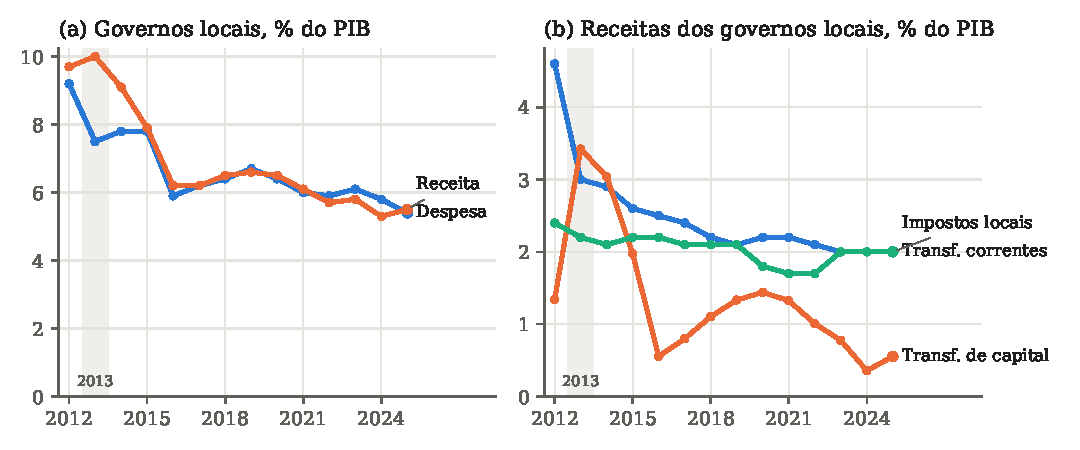
\includegraphics[width=\textwidth]{figuras/fig_hungria_local.pdf}
  \caption{Hungria: tamanho e receitas dos governos locais (2012--2025)}
  \label{fig:hungria}
  \fonte{elaboração própria com dados do Eurostat (gov\_10a\_main). A faixa cinza marca 2013.}
\end{figure}

A leitura do financiamento exige separar as transferências de capital. Em 2013 e 2014, a receita local (10,0\% e 9,1\% do PIB) superou a despesa (7,5\% e 7,8\%), porque o setor recebeu transferências de capital de 3,4\% e 3,0\% do PIB, que correspondem, provavelmente, à assunção das dívidas municipais pelo governo central \citep{Bethlendi2018, Racz202191}. Incluídas essas transferências, a participação das transferências na receita sobe de 61,7\% em 2012 para 64,6\% em 2013 e só depois cai, até 47,1\% em 2025. Em proporção do PIB, o quadro é mais limpo: as transferências correntes recebidas caíram de 4,6\% para 2,0\% do PIB entre 2012 e 2025, enquanto os impostos locais ficaram entre 1,7\% e 2,4\%, apoiados no imposto sobre atividades econômicas \citep{Kecso2020}. Medida sem as transferências de capital no denominador, a participação das transferências correntes caiu de 55,5\% em 2012 para 39\% a 47\% a partir de 2013, sem tendência clara depois de 2019.

A hipótese H3 é, portanto, rejeitada na forma em que foi enunciada, com a ressalva de que ela era teoricamente ambígua. Ao assumir escolas e outros serviços, o Estado deixou de transferir os recursos que os financiavam, e a razão entre transferências e receita caiu porque funções e recursos saíram juntos, ao contrário do caso polonês, em que a recentralização elevou o peso das transferências \citep{Poniatowicz202489}. A literatura sobre a segunda onda indica que o instrumento de controle passou a ser a parcela discricionária das transferências, distribuída segundo o alinhamento político \citep{Vasvari2024467, Vasvari20241371, Kovarek2023}, e os dados agregados do Eurostat não separam essa parcela. Os instrumentos descritos na Seção~\ref{sec:hungria_lit}, o financiamento por tarefa e a contribuição de solidariedade, reduzem o controle local sobre a receita sem aparecer como aumento de dependência, porque o primeiro retira funções e o segundo é uma saída de recursos. O relatório do Índice de Autonomia Local registra a consequência dentro do período da série: a Hungria foi um dos dois únicos países com queda expressiva no escopo de competências locais, quando os escritórios distritais criados em 2013 assumiram parte da assistência social e da educação básica \citep{LAIreport}. Menos dependência veio, assim, acompanhada de menos competências, o que apoia H4 no sentido húngaro. As razões húngaras e brasileiras têm definições diferentes e não são comparáveis em nível; o contraste está na direção dos movimentos, não na comparação dos percentuais.

\subsection{O que mudou em relação ao trabalho anterior}

Os resultados acima dependem de uma base corrigida, e as correções também têm consequências próprias. A atualização partiu do trabalho anterior \citep{DutraP1}, cuja cópia integral foi preservada no repositório. Dos 340 valores municipais comparáveis (17 variáveis, dois municípios, 2014--2023), 327 coincidem com a nova coleta, nove foram corrigidos e quatro, antes ausentes, foram preenchidos. A Tabela~\ref{tab:alteracoes} resume as alterações.

\begin{table}[H]
\centering\footnotesize
\setlength{\tabcolsep}{4pt}
\caption{Principais alterações em relação ao trabalho anterior (2014--2023)}
\label{tab:alteracoes}
\begin{adjustbox}{max width=\textwidth}
\begin{tabular}{p{3.3cm}p{2.1cm}p{6.2cm}r}
\toprule
Variável & Anos & Alteração & Diferença \\
\midrule
Receita total (Camaçari) & 2019--2023 & A base original excluía as receitas intraorçamentárias, mas não as despesas & +1,8 a +5,5\% \\
FPM & Bar. 2016, Cam. 2017 & A base original omitia as parcelas de 1\% & +0,4 a +9,0\% \\
Despesa em saúde (Camaçari) & 2019 & A base original registrava zero; valor da DCA: R\$ 239,3 mi & -- \\
População (Barreiras) & 2018 & Erro de digitação na base original (158.331; IBGE: 153.831) & -2,8\% \\
População & 2022--2023 & Ausente na base original; Censo 2022 e interpolação & -- \\
Resultado orçamentário & 2014--2023 & A base original não descontava a dedução do FUNDEB da receita (R\$ 28 a 158 mi/ano); superávit vira déficit em 7 município-anos (Bar. 2014, Bar. 2015, Bar. 2020, Bar. 2022, Bar. 2023, Cam. 2014, Cam. 2015); ver Tabela~\ref{tab:resultado} & -- \\
Despesa por função & vários & Zeros da base original tratados como ausentes & -- \\
Hungria: receita e despesa do gov. geral & 2014--2021 & A base original trazia estimativas em HUF; a atualização usa o valor oficial do Eurostat & -7,5 a +7,5\% \\
Ampliações & 2014--2025 & 2024--2025; ITR, IPVA, IPI, SUS, deduções do FUNDEB; governos locais húngaros & -- \\
\bottomrule
\end{tabular}
\end{adjustbox}
\par\vspace{3pt}\parbox{\textwidth}{\scriptsize Nota: dos 340 valores municipais comparáveis (17 variáveis, 2 municípios, 2014--2023), 327 coincidem com a base original (diferença menor que 0,1\%). Diferença = (valor novo $-$ valor original)/valor original. Registro completo em data/registro\_alteracoes/. Fonte: elaboração própria.}
\end{table}


A correção de maior consequência é a do resultado orçamentário, detalhada na Tabela~\ref{tab:resultado}. O trabalho anterior o calculou com a receita bruta, sem descontar a dedução para a formação do FUNDEB, de R\$~28 a 158 milhões por ano. Com a correção, o superávit apontado anteriormente vira déficit em sete município-anos entre 2014 e 2023: cinco em Barreiras (2014, 2015, 2020, 2022 e 2023) e dois em Camaçari (2014 e 2015). Somados os anos de 2018 e 2019, já deficitários no cálculo bruto, Barreiras registra resultado de execução negativo em sete dos dez anos de 2014 a 2023. O resultado de um exercício, porém, não mede sozinho a situação fiscal: não considera restos a pagar, disponibilidade de caixa nem superávits financeiros de exercícios anteriores, que podem financiar déficits de execução sem desequilíbrio. A conclusão correta é mais estreita do que ``Barreiras é deficitária'': a leitura de equilíbrio orçamentário persistente do trabalho anterior não se sustenta.

\begin{table}[H]
\centering\footnotesize
\setlength{\tabcolsep}{4pt}
\caption{Resultado orçamentário com e sem a dedução para o FUNDEB (R\$ milhões correntes)}
\label{tab:resultado}
\begin{adjustbox}{max width=\textwidth}
\begin{tabular}{lrrrrrr}
\toprule
 & \multicolumn{3}{c}{Barreiras} & \multicolumn{3}{c}{Camaçari} \\
\cmidrule(lr){2-4}\cmidrule(lr){5-7}
Ano & Bruto & Dedução & Líquido & Bruto & Dedução & Líquido \\
\midrule
2014 & 17,2 & 27,9 & -10,7$^{\dagger}$ & 81,9 & 88,9 & -7,0$^{\dagger}$ \\
2015 & 19,9 & 30,6 & -10,7$^{\dagger}$ & 80,2 & 98,4 & -18,2$^{\dagger}$ \\
2016 & 43,5 & 32,4 & 11,2 & 189,7 & 104,2 & 85,5 \\
2017 & 212,4 & 32,9 & 179,5 & 218,4 & 103,6 & 114,9 \\
2018 & -40,6 & 35,8 & -76,4 & 151,8 & 114,7 & 37,1 \\
2019 & -23,6 & 38,7 & -62,2 & 172,7 & 126,9 & 45,8 \\
2020 & 32,1 & 39,9 & -7,7$^{\dagger}$ & 227,1 & 124,4 & 102,6 \\
2021 & 74,1 & 52,3 & 21,8 & 184,4 & 145,2 & 39,2 \\
2022 & 20,7 & 63,7 & -43,1$^{\dagger}$ & 196,4 & 155,5 & 40,9 \\
2023 & 56,0 & 69,8 & -13,8$^{\dagger}$ & 288,4 & 157,8 & 130,6 \\
2024 & 88,0 & 81,8 & 6,2 & 176,6 & 157,6 & 19,0 \\
2025 & 47,8 & 89,3 & -41,6$^{\dagger}$ & 244,4 & 167,8 & 76,6 \\
\bottomrule
\end{tabular}
\end{adjustbox}
\par\vspace{3pt}\parbox{\textwidth}{\scriptsize Nota: Bruto = receita total bruta menos despesa empenhada, como no trabalho anterior; Líquido = receita total líquida da dedução para a formação do FUNDEB menos despesa empenhada. $\dagger$ = superávit no cálculo bruto que vira déficit no líquido. Entre 2014 e 2023, o resultado líquido é negativo em 7 anos em Barreiras (2014, 2015, 2018, 2019, 2020, 2022, 2023) e em 2 em Camaçari (2014, 2015). O resultado da execução de um exercício não mede, isoladamente, a situação fiscal: não considera restos a pagar, disponibilidade de caixa nem superávits financeiros de exercícios anteriores. Fonte: elaboração própria com dados do Siconfi (DCA).}
\end{table}


Outras correções afetam definições. A receita de Camaçari entre 2019 e 2023 excluía as receitas intraorçamentárias, mas não as despesas correspondentes; o FPM de 2016 e 2017 omitia as parcelas adicionais de 1\%; a despesa em saúde de Camaçari em 2019 aparecia como zero, quando foi de R\$~239,3 milhões; e a população de Barreiras em 2018 tinha dígitos trocados. Para a Hungria, os valores do governo geral em moeda nacional entre 2014 e 2021 eram estimativas, com diferenças de até 7,5\% em relação aos dados oficiais.

A atualização também ampliou a base: incluiu 2024 e 2025, separou as transferências por origem e tipo, incorporou as deduções do FUNDEB e os dados dos governos locais húngaros e substituiu a regressão anterior, que relacionava receita e PIB e juntava municípios de escalas muito diferentes, pelo modelo de efeitos marginais com efeito fixo, testes de robustez e placebos. Um registro merece destaque. Em 2017, Barreiras recebeu R\$~178,6 milhões em ``Outras Transferências Multigovernamentais'', valor que não se repete em nenhum outro ano e equivale a 31,5\% da receita total bruta do exercício, de R\$~567,8 milhões. O valor foi mantido, por ser oficial, mas isolado nas análises de dependência; nas regressões, ele não entra nas transferências incondicionais, e a retirada de 2017 não altera os resultados (Tabela~\ref{tab:robustez}). Sua natureza não foi confirmada em fonte primária e merece verificação.
